\documentclass[compress]{beamer}
\usepackage{ifthen,verbatim}

\newcommand{\isnote}{}
\xdefinecolor{lightyellow}{rgb}{1.,1.,0.25}
\xdefinecolor{darkblue}{rgb}{0.1,0.1,0.7}

%% Uncomment this to get annotations
%% \def\notes{\addtocounter{page}{-1}
%%            \renewcommand{\isnote}{*}
%% 	   \beamertemplateshadingbackground{lightyellow}{white}
%%            \begin{frame}
%%            \frametitle{Notes for the previous page (page \insertpagenumber)}
%%            \itemize}
%% \def\endnotes{\enditemize
%% 	      \end{frame}
%%               \beamertemplateshadingbackground{white}{white}
%%               \renewcommand{\isnote}{}}

%% Uncomment this to not get annotations
\def\notes{\comment}
\def\endnotes{\endcomment}

\setbeamertemplate{navigation symbols}{}
\setbeamertemplate{headline}{\mbox{ } \hfill
\begin{minipage}{5.5 cm}
\vspace{-0.75 cm} \small
\end{minipage} \hfill
\begin{minipage}{4.5 cm}
\vspace{-0.75 cm} \small
\begin{flushright}
\ifthenelse{\equal{\insertpagenumber}{1}}{}{Jim Pivarski \hspace{0.2 cm} \insertpagenumber\isnote/\pageref{numpages}}
\end{flushright}
\end{minipage}\mbox{\hspace{0.2 cm}}\includegraphics[height=1 cm]{../cmslogo} \hspace{0.01 cm} \vspace{-1.05 cm}}

\begin{document}
\begin{frame}
\vfill
\begin{center}
\textcolor{darkblue}{\Large Combining HW+TB endcap alignment}

\vfill
\begin{columns}
\column{0.75\linewidth}
\begin{center}
\large
Jim Pivarski
\end{center}
\end{columns}

\vfill
23 July, 2010

\end{center}
\end{frame}

%% \begin{notes}
%% \item This is the annotated version of my talk.
%% \item If you want the version that I am presenting, download the one
%% labeled ``slides'' on Indico (or just ignore these yellow pages).
%% \item The annotated version is provided for extra detail and a written
%% record of comments that I intend to make orally.
%% \item Yellow notes refer to the content on the {\it previous} page.
%% \item All other slides are identical for the two versions.
%% \end{notes}

\small

\begin{frame}
\frametitle{General idea}
\begin{columns}
\column{0.5\linewidth}
\begin{itemize}
\item Track-based CSC alignment module optimizes alignment given a set of measurements (positions with independent uncertainties)
\item Some of these are derived from track residuals; others may be introduced by hand (e.g.\ photogrammetry)
\item Only requirement is that there must be enough measurements that the graph is fully connected (no islands)
\item Adding DCOPS: we would add 3 new floating coordinate frames connected to the monitored chambers
\end{itemize}

\column{0.5\linewidth}
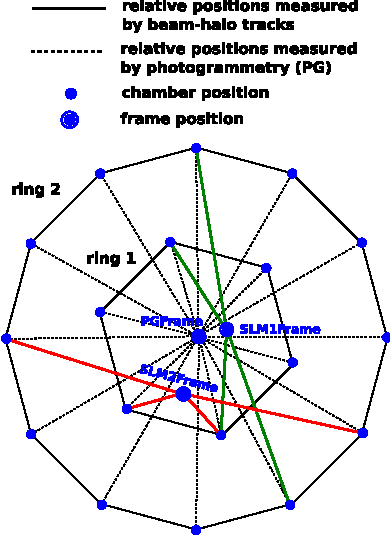
\includegraphics[width=\linewidth]{beamhalo-PG-SLM.pdf}
\end{columns}
\end{frame}

\begin{frame}[fragile]
\frametitle{Technical details}
\begin{itemize}
\item Adding measurement ``lines'' to the graph: this is in the CMSSW configuration file--- I would do it

\item Providing measurements:
\begin{itemize}
\item two simple-format text files: see \mbox{\href{http://cmssw.cvs.cern.ch/cgi-bin/cmssw.cgi/CMSSW/Alignment/MuonAlignmentAlgorithms/data}{\textcolor{blue}{Alignment/MuonAlignmentAlgorithms/data/Photogrammetry2007.*}}\hspace{-2 cm}}
\begin{verbatim}
ME+1/2/01 -3.9173832602512e-05 5.73795e-05
ME+1/2/02 0.174428948607051 5.73795e-05
ME+1/2/03 0.348821455510375 5.73795e-05
...
\end{verbatim}
\item ``phipos'' file: $\phi = \mbox{atan2}(Y, X)$ position and uncertainty of each monitored chamber in disk coordinates (radians)
\item ``phiz'' file: $\phi_z$ angle and uncertainty of each monitored chamber (radians)
\end{itemize}
\item Automated machinery takes over from there
\item We can check consistency via the alignment fit residuals, but it's worth checking against the Photogrammetry2007.* files to make sure that we're using the same conventions
\end{itemize}
\end{frame}

\begin{frame}
\begin{center}
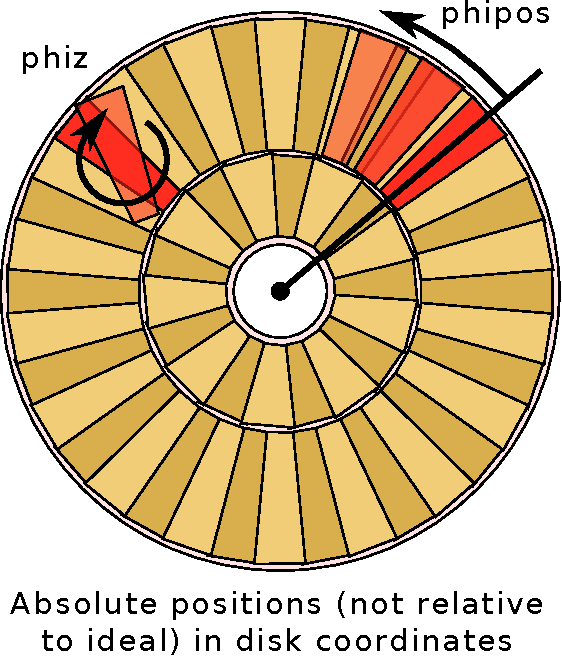
\includegraphics[width=0.5\linewidth]{diagram.pdf}
\end{center}
\label{numpages}
\end{frame}

%% \begin{frame}
%% \frametitle{Outline}
%% \begin{itemize}\setlength{\itemsep}{0.75 cm}
%% \item 
%% \end{itemize}
%% %% \hspace{-0.83 cm} \textcolor{darkblue}{\Large Outline2}
%% \end{frame}

%% \section*{First section}
%% \begin{frame}
%% \begin{center}
%% \Huge \textcolor{blue}{First section}
%% \end{center}
%% \end{frame}

%% \begin{frame}
%% \end{frame}

\end{document}
